\documentclass[10pt]{article}
\usepackage{icmlko}

\icmlmeta{IP 파운데이션 월드모델}{343}{여섯 번째 목록}{모바일 태그 축이 한 번도 안 만들어지고 있었다 --- 그리고 검사 ⑤ 가 판 이득을 소수 넷째 자리까지 맞혔다}

\begin{document}

\twocolumn[
\icmlheader

\begin{abstract}
노트 342가 ``새 축 후보에 검사 ⑤ 를 --- 붙이기 전에''를 갈래 머리에 뒀다.
후보를 찾다가 \textbf{여섯 번째 갈라진 목록}을 만났다 ---
\texttt{lab/tagaxes.FIELDS} 에는 모바일이 있는데 \texttt{SPEC} 에는 없다.
\texttt{SPEC} 이 어느 도메인에 축을 만들지 정하므로 \textbf{모바일 태그
축은 한 번도 안 만들어졌다.}

만들어 봤다. 학습 1,559행 · 토큰 46종. 성분 넷 중 셋이 검사 ①②를
통과하고($\rho$ $+$0.262 · $-$0.260 · $+$0.321 · 조각 다 5/5),
\textbf{검사 ③ 에서 성분 0 이 \texttt{target\_breadth} 와 0.814 로
떨어진다} --- 언어 수는 이미 넓이 축이다. 남은 (2,3)이 후보다.

\textbf{그리고 붙이기 전에 검사 ⑤ 를 돌렸다} --- 이 도구의 첫 실사용이다.

\begin{center}\small
\begin{tabular}{lrr}
\hline
 & 검사 ⑤ (붙이기 전) & 실제 (붙이고) \\
\hline
\textbf{판} & \textbf{$+$0.0042 (8/8)} & \textbf{$+$0.0041 (11/12)} \\
모바일 & $+$0.0290 (8/8) & $+$0.0305 (12/12) \\
\hline
\end{tabular}
\end{center}

\textbf{검사 ⑤ 가 판 이득을 소수 넷째 자리까지 맞혔다.} 노트 341이
``검사 ⑤ 는 붙일까에 답하지 뺄까에는 답하지 않는다''로 경계를 그었는데,
\textbf{붙이는 쪽에서는 정말로 답한다.}

배포 규칙 ①② 를 통과한다 --- 판이 미결정 폭 안이고(부호는 11/12 로 선다)
제일 나쁜 도메인이 게임 $-$0.0064(짝SE 0.03 · $t{\approx}0.2$)다.
\textbf{채택한다.}
\end{abstract}
]

\section{여섯 번째 목록}

\begin{center}\footnotesize
\begin{tabular}{lll}
\hline
 & 어디 & 노트 \\
\hline
거르는 쪽 & \texttt{ingest/idol\_axes} & 326 \\
긁는 쪽 & \texttt{wiki\_views.idol\_items} & 332 \\
 & \texttt{idol\_album\_meta.run} & 333 \\
읽는 쪽 & \texttt{trendaxes.FILE} & 336 \\
 & \texttt{wikiaxes.AXF} & 337 \\
\textbf{만드는 쪽} & \texttt{tagaxes.SPEC} & \textbf{343} \\
\hline
\end{tabular}
\end{center}

\texttt{FIELDS} 는 ``이 도메인에서 토큰을 어디서 모으나''이고
\texttt{SPEC} 은 ``이 도메인에 축을 만드나''다. 모바일은 앞에만 있었다 ---
\textbf{토큰을 모을 줄은 아는데 축은 안 만든다.}

\begin{figure*}[t]
\centering
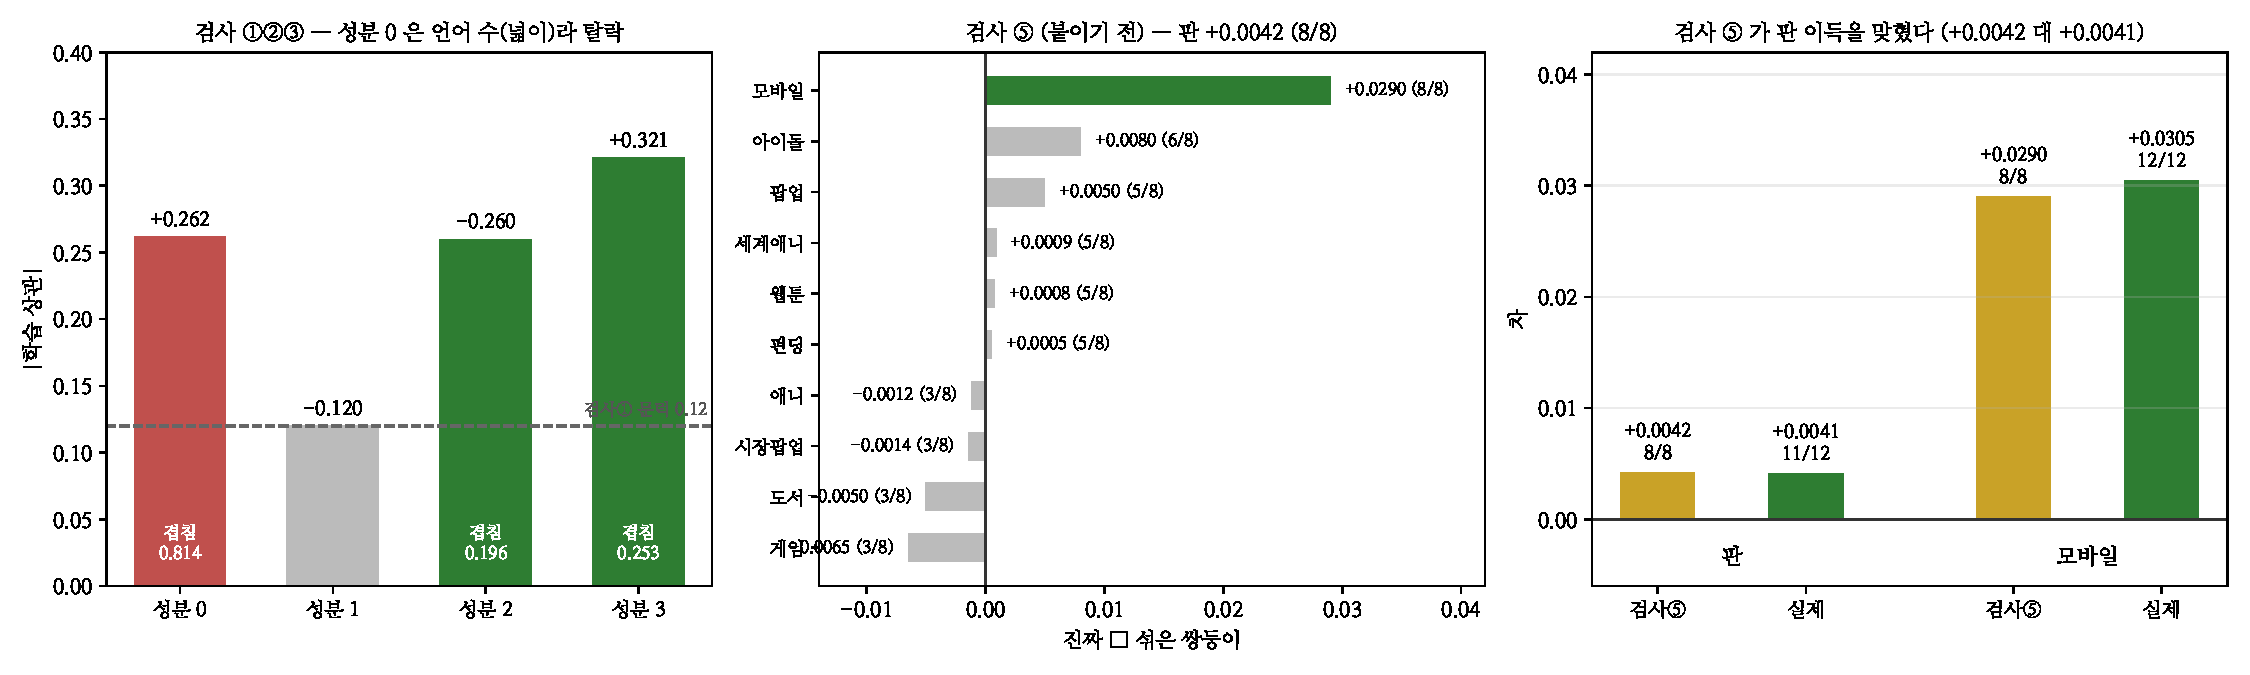
\includegraphics[width=\textwidth]{figs/sixth.pdf}
\caption{왼쪽 --- 검사 ①②③. 가운데 --- 검사 ⑤. 오른쪽 --- 예측과 실제.}
\end{figure*}

\section{검사 ①②③}

\begin{center}\footnotesize
\begin{tabular}{lrrl}
\hline
성분 & 학습 $\rho$ & 최대 겹침 & 판정 \\
\hline
0 & $+$0.262 & \textbf{0.814} (\texttt{target\_breadth}) & \textbf{탈락} \\
1 & $-$0.120 & --- & ① 아슬 \\
\textbf{2} & $-$0.260 & 0.196 & \textbf{통과} \\
\textbf{3} & $+$0.321 & 0.253 & \textbf{통과} \\
\hline
\end{tabular}
\end{center}

성분 0 에 실린 토큰이 \texttt{l:FR} · \texttt{l:DE} · \texttt{l:JA} ·
\texttt{l:IT} 다 --- \textbf{몇 개 언어로 냈나}이고 그것이 곧 넓이다.
\textbf{검사 ③ 이 제 일을 했다.} 남은 둘은 장르 쪽이다(성분 2 는
\texttt{g:엔터테인먼트} $+$0.70 · \texttt{g:보드} $+$0.35 · \texttt{l:KO}
$-$0.26).

\section{붙이기 전에 검사 ⑤}

\begin{center}\footnotesize
\begin{tabular}{lrr}
\hline
도메인 & 진짜 $-$ 쌍둥이 & 양수 \\
\hline
\textbf{모바일} & \textbf{$+$0.0290} & \textbf{8/8} \\
아이돌 & $+$0.0080 & 6/8 \\
팝업 & $+$0.0050 & 5/8 \\
게임 & $-$0.0065 & 3/8 \\
\hline
\textbf{판} & \textbf{$+$0.0042} & \textbf{8/8} \\
\hline
\end{tabular}
\end{center}

\textbf{제 도메인에서 8/8 로 이긴다.} 노트 339가 잰 ``잡음 축은 판을
0.126 내린다''를 생각하면, 이 축은 그 값을 물고도 $+$0.0042 를 남긴다.

\section{붙였다}

\begin{center}\footnotesize
\begin{tabular}{lrrr}
\hline
 & 평균 & SD & 양수 \\
\hline
\textbf{판} & \textbf{$+$0.0041} & 0.0025 & \textbf{11/12} \\
\textbf{모바일} & \textbf{$+$0.0305} & 0.0120 & \textbf{12/12} \\
시장팝업 & $-$0.0120 & 0.0244 & 5/12 \\
게임 & $-$0.0064 & 0.0098 & 2/12 \\
도서 & $-$0.0050 & 0.0222 & 5/12 \\
\hline
\end{tabular}
\end{center}

\textbf{판 기준값이 0.4642 $\to$ 0.4694 다.} 크기는 미결정 폭 안이지만
SD 가 0.0025 라 \textbf{부호가 선다}(11/12) --- 노트 329가 세운 대로
축만 바꾸는 짝은 부호를 믿을 수 있다.

\paragraph{검사 ⑤ 가 맞혔다} 판 $+$0.0042 대 $+$0.0041, 모바일
$+$0.0290 대 $+$0.0305. \textbf{두 자리 다 소수 넷째 자리에서 만난다.}
노트 341이 ``검사 ⑤ 는 뺄까에 답하지 않는다''고 경계를 그었고, 오늘
\textbf{붙일까에는 답한다}가 확인됐다.

\section{남은 것}
\begin{center}\footnotesize
\begin{tabular}{ll}
\hline
갈래 & 왜 \\
\hline
\textbf{만드는 쪽 목록을 다 대조} & 여섯 번째다 --- \texttt{listaudit} 에 \\
게임 · 도서 태그 & \texttt{FIELDS} 에 없다 --- 토큰이 있나 \\
시장팝업이 왜 또 $-$0.012 & 노트 342에서도 다 졌다 \\
검사 ⑤ 를 후보 전부에 & 이제 붙이기 전에 쓴다 \\
\hline
\end{tabular}
\end{center}

\paragraph{규약} \textbf{도구를 만들었으면 다음 후보에 바로 써라.} 검사 ⑤
를 노트 341에 만들고 342에서 지도를 그렸는데, 그 둘은 다 \emph{이미 붙인}
축에 돌린 것이었다. 오늘 처음으로 \textbf{안 붙인 후보}에 돌렸고 거기서
값이 났다 --- 판 이득을 미리 맞혔다. \textbf{그리고 후보는 새로 만들어서
찾은 게 아니라 갈라진 목록에서 나왔다} --- 여섯 번째다. \textbf{이 판에서
제일 싼 개선은 아직도 ``이미 있는 것을 다 쓰고 있나''를 세는 일이다.}

\end{document}
